\section{LPython}

\begin{frame}{LPython - Motivation}
    \begin{itemize}
        \item Python - long favoured for simplicity, intuitive syntax, productivity, ecosystem
        \item But inherently slow compared to other compiled langauges such as C and C++.
        \item LPython - Type Annotated Python Compiler for performance
        % \item Other compilers like Cython, Mojo, Numba, Pytorch exist. Why LPython?
        % \begin{itemize}
        %     \item Cython generates C code, but calls into Python for most Python features. Mojo is a superset, not compatible with CPython. Numba can't do ahead of time. PyTorch is only for AI stuff. 
        % \end{itemize}
        \item Most existing Python compilers focus on improving Python performance
        \item LPython aims to run Python at the maximum possible speed
    \end{itemize}
\end{frame}

\begin{frame}{LPython compared to C++}
    \begin{columns}
        \scalebox{.25}{
        \begin{column}{1.6\textwidth}
            \lstinputlisting[language=Python]{codes/dijkstra-code.py}
        \end{column}
        }
        \begin{column}{0.6\textwidth}
            \begin{figure}
                \centering
                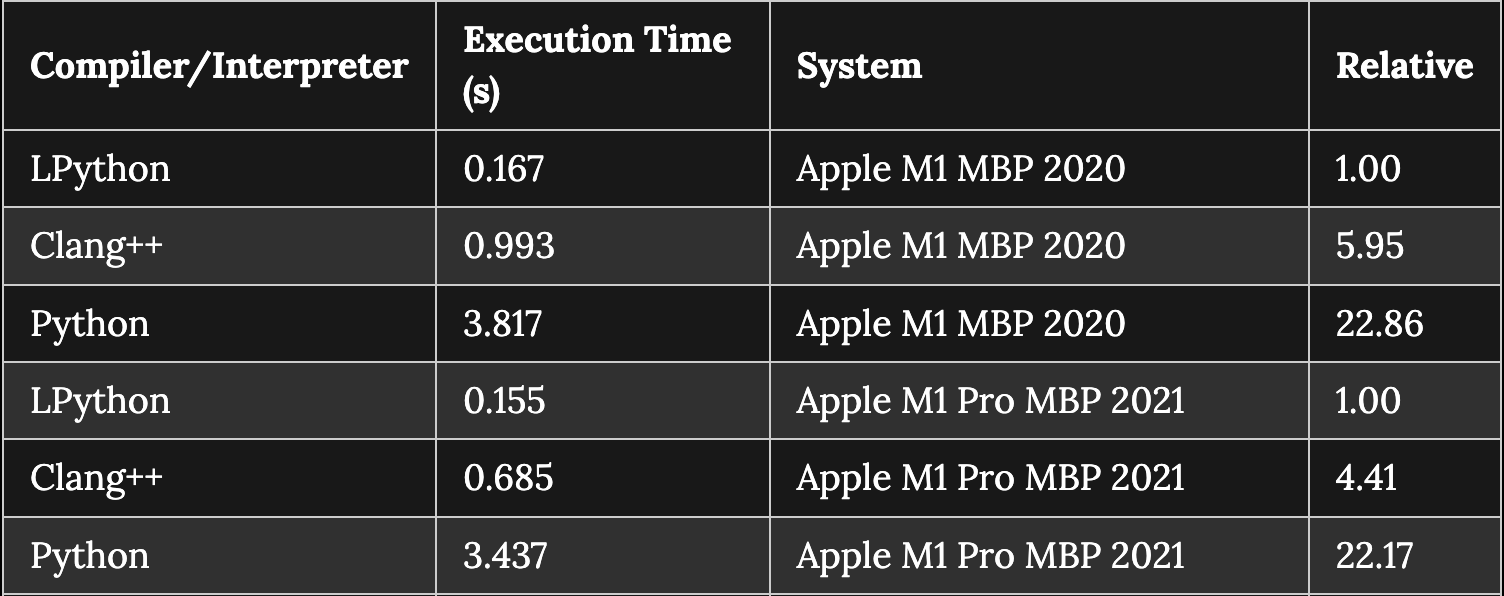
\includegraphics[width=7cm]{images/benchmark.png}
            \end{figure}
            \scriptsize \centering Note that the following optimization flags were used:
            \begin{figure}
                \centering
                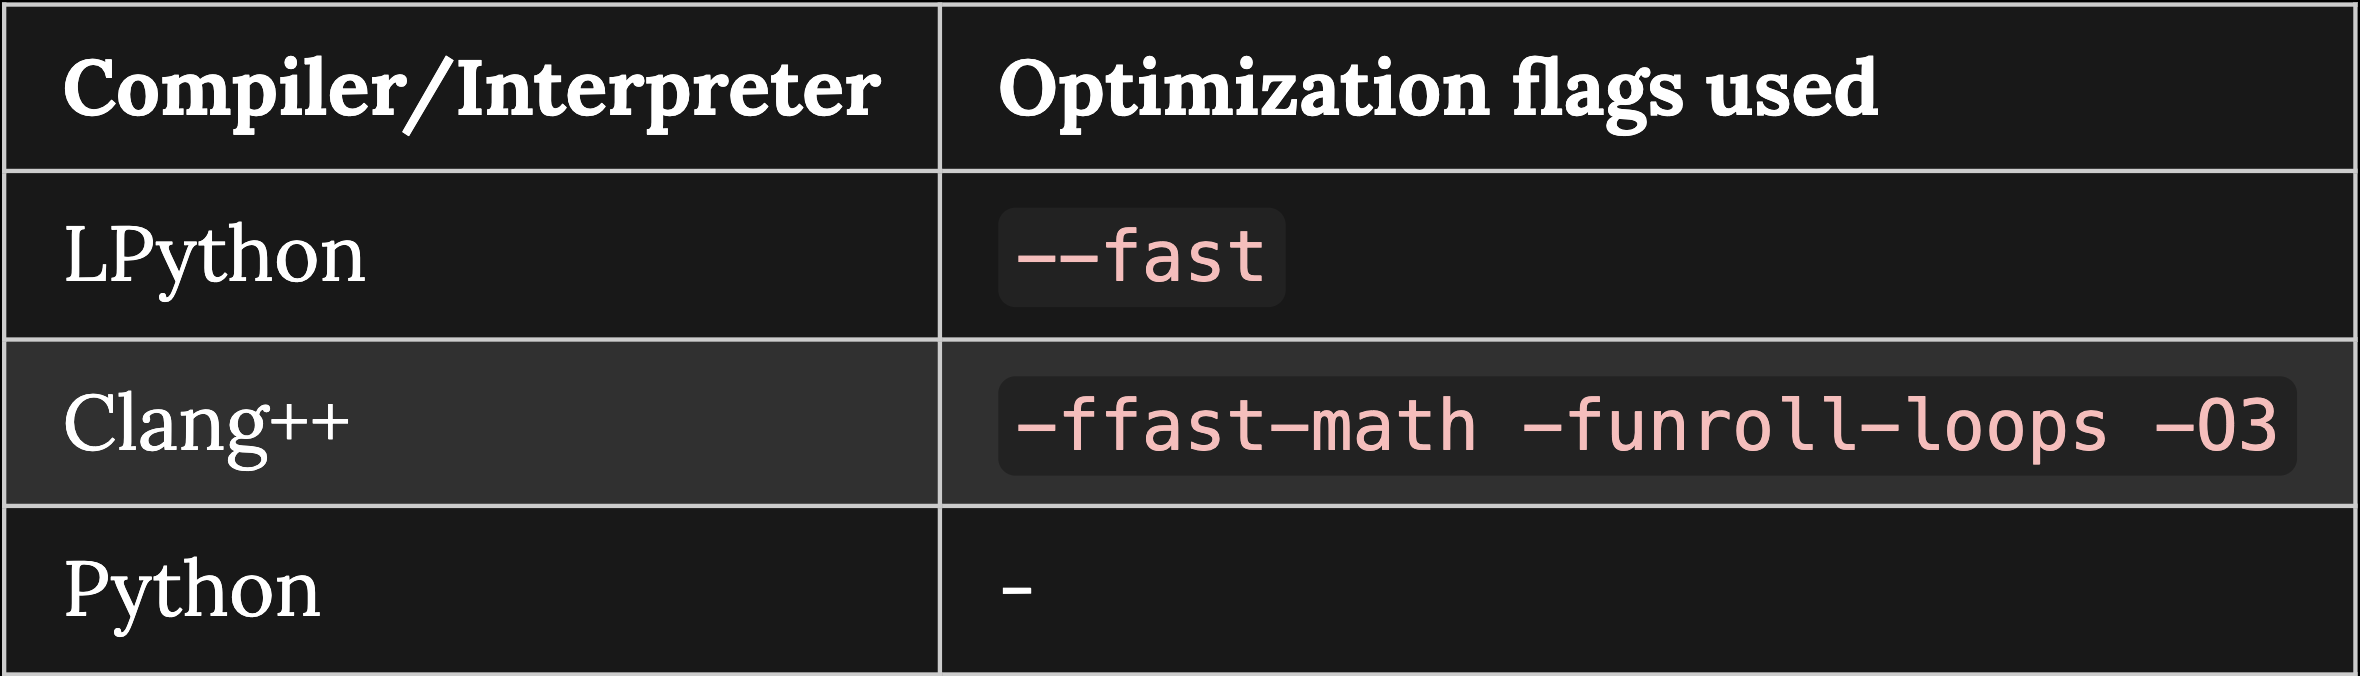
\includegraphics[width=5cm]{images/optimization-flags.png}
            \end{figure}
        \end{column}
    \end{columns}
    \scriptsize
    More Benchmarks at \href{https://lpython.org/blog/2023/07/lpython-novel-fast-retargetable-python-compiler/}{https://lpython.org/blog/2023/07/lpython-novel-fast-retargetable-python-compiler/}
\end{frame}

\begin{frame}{Star History}
    \begin{figure}
        \centering
        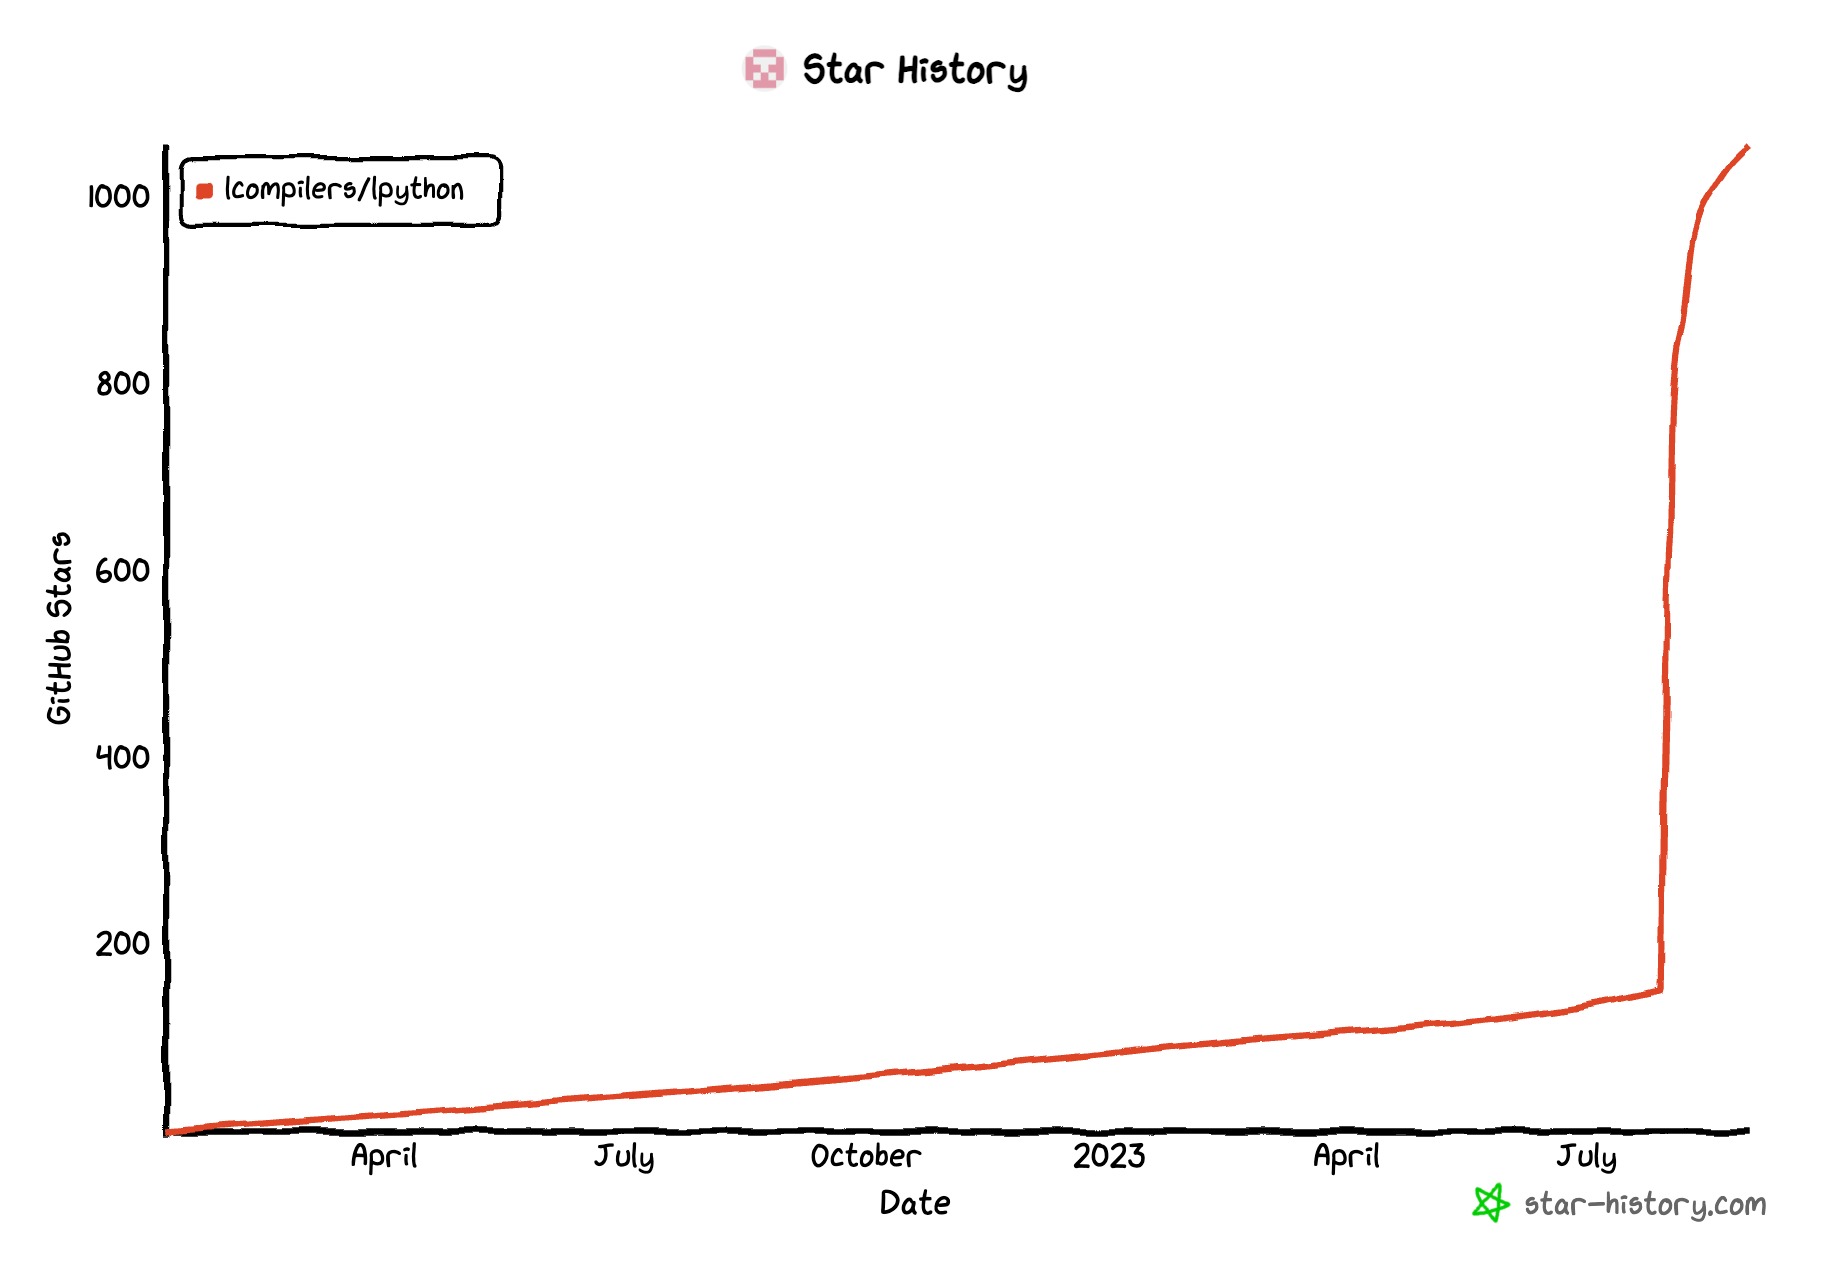
\includegraphics[width=8cm]{images/star-history.png}
        \caption{Spike in star count when we released LPython alpha}
    \end{figure}   
\end{frame}

\begin{frame}{LPython}
    \begin{columns}
        \begin{column}{0.5\textwidth}
            \scriptsize
            \lstinputlisting[language=Python]{codes/type-annotated-example.py}
            \centering Type annotated example code
        \end{column}
        \begin{column}{0.5\textwidth}
            \begin{itemize}
                \item Supports subset of CPython
                \item Requires types (annotations)
                \item If LPython compiles and runs, it will run in CPython
                \item Never slower than C and C++
                \begin{itemize}
                    \item \tiny{If you find an example where it is slower, it is a bug and we request you to report it to us.}
                \end{itemize}
                \item Several backends: LLVM, C, C++, WASM, X64 (via WASM)
            \end{itemize}
        \end{column}
    \end{columns}
\end{frame}
